\section{Class 2 - 26/02/21}
\subsection*{Vector wave equation}
Here we go again, today from \cref{eq:maxwell_system} we want to obtain the wave equation of the EMF, we will make a lot of simplification.\\
First of all we consider:
\begin{itemize}
    \item No accumulated charge (source free, no current that generates the EMF) $\boldsymbol{\overline{J_i}=0}$
    \item No losses (nonconducting medium) $\boldsymbol{\overline{J_i}$ $\sigma \cdot\overline{E}}$
\end{itemize}
Then from \cref{eq:maxwell_system} we now have:
\begin{equation}\label{eq:maxwell_simplified}
    \begin{cases}
    \nabla\times\overline{E}=-\mu\frac{\partial \overline{H}}{\partial t}\\[5pt]
    \nabla\times\overline{H}=\varepsilon\frac{\partial \overline{E}}{\partial t}
    \end{cases}
\end{equation}
We continue to try to find the wave equation by using some tricks, the next passage is to apply the curl on the first equation from \cref{eq:maxwell_simplified}.
\begin{align}
    \begin{split}
        \nabla\times\nabla\times\overline{E}=&-\nabla\times\mu \frac{\partial \overline{H}}{\partial t}=-\mu \frac{\partial}{\partial t} \nabla\times \overline{H}\\[5pt]
        &=-\mu \frac{\partial}{\partial t}\varepsilon\frac{\partial \overline{E}}{\partial t}=\\[5pt]
        &=-\mu \varepsilon \frac{\partial^2\overline{E}}{\partial t^2}
    \end{split}
\end{align}
We remember a cool property of the curl of a curl of a vector field:
\begin{equation}
    \nabla\times\nabla\times\overline{E}=\nabla(\nabla\cdot \overline{E})-\nabla^2\,\overline{E}
\end{equation}
Please note that we have already discussed the $\nabla^2$ symbol before in \cref{sec:laplacian} as the Laplacian. Now let's write:
\begin{equation}
    \nabla(\nabla\cdot \overline{E})-\nabla^2\,\overline{E}=-\mu \varepsilon \frac{\partial^2\overline{E}}{\partial t^2}
\end{equation}
We simplify a little bit more, and we consider that we don't have free charge: $\nabla(\varepsilon \overline{E}=0)$ and we obtain:
\begin{equation}\label{eq:whave_1}
    \nabla^2\,\overline{E}-\mu \varepsilon \frac{\partial^2\overline{E}}{\partial t^2}=0
\end{equation}
WE FINALLY OBTAINED THE \emph{WAVE EQUATION}. Here we define a constant that will be helpful next:
\begin{equation}
    c=\frac{1}{\sqrt{\mu\varepsilon}}
\end{equation}
Then \cref{eq:whave_1} becomes:
\begin{equation}\label{eq:whave_2}
    \nabla^2\,\overline{E}-\frac{1}{c^2} \frac{\partial^2\overline{E}}{\partial t^2}=0
\end{equation}
Pay attention to one thing: if you look at the maxwell equation \cref{eq:maxwell_simplified} it is a differential equation of the first order, but now we have a second order differential equation (\cref{eq:whave_2}) and the set of solution is increased. We don't address this problem now, but keep in mind that later we will be able to select the good solution by using the divergence equation (\textsl{i don't really know what does it mean}).\\
If instead use the second equation from \cref{eq:whave_2}, and we do all the passages as before, we obtain nearly the same equation, but with $\overline{H}$
\begin{equation}
    \nabla^2\,\overline{H}-\frac{1}{c^2} \frac{\partial^2\overline{H}}{\partial t^2}=0
\end{equation}
\subsection*{Scalar wave equation}
Now let's try to write our equation with scalars and not vectors, it should simplify a bit.\\
If we consider the vector $E$ to be completely parallel to the $z$ axes, it means:
\begin{equation}
    \overline{E}(x,y,z)=\xcancel{E_x\ihat}+\xcancel{E_y\jhat}+E_z\khat\;\rightarrow \:\overline{E}(x,y,z)=E(z)
\end{equation}
But actually $E$ is also dependent on time, so we deal with: $E(z,t)$\\
Now \cref{eq:whave_2} with scalar $E$ becomes:
\begin{equation}\label{eq:whave_simplified}
    \frac{\partial^2E}{\partial z^2}-\frac{1}{c^2} \frac{\partial^2E}{\partial t^2}=0
\end{equation}
\subsubsection*{Solution of the scalar wave equation}
Searching for the solution of \cref{eq:whave_simplified} is a bit time consuming, but it should have the shape of:
\begin{equation}
    E(z,t)=f_1\left(t-\frac{z}{c}\right)+f_2\left(t+\frac{z}{c}\right)
\end{equation}
So without going into tedious calculation, we look at 2 possible solutions for $f_1$ and $f_2$:
\begin{align}\label{eq:maxwell_solution_simple}
    \begin{split}
        &E_1(z,t)=E_0 \cos\left[\omega\left(t-\frac{z}{c}\right)\right]\\[5pt]
        &E_2(z,t)=E_0 \cos\left[\omega\left(t+\frac{z}{c}\right)\right]
    \end{split}
\end{align}
Does that satisfy the maxwell equation? Let's consider the first solution of \cref{eq:maxwell_solution_simple} and verify that it actually satisfy \cref{eq:whave_simplified}:
\begin{align*}
    \begin{split}
        \frac{\partial^2E}{\partial z^2}=&\frac{\partial}{\partial z}\left\{E_0\left[-\left(-\frac{\omega}{c}\right)\sin\left[\omega\left(t-\frac{z}{c}\right)\right]\right]\right\}=\\[5pt]
        =&E_0\,\frac{\omega}{c}\left\{\left(-\frac{\omega}{c}\right)\cos\left[\omega\left(t-\frac{z}{c}\right)\right]\right\}=\\[5pt]
        =&-E_0\,\frac{\omega^2}{c^2}\cos\left[\omega\left(t-\frac{z}{c}\right)\right]\\[10pt]
        \frac{\partial^2E}{\partial t^2}=&\frac{\partial}{\partial t}\left\{E_0\left[-\omega\, \sin\left[\omega\left(t-\frac{z}{c}\right)\right]\right]\right\}=\\[5pt]
        =&-E_0\,\omega\left\{\omega \, \cos\left[\omega\left(t-\frac{z}{c}\right)\right]\right\}=\\[5pt]
        =&-E_0\,\omega^2\,\cos\left[\omega\left(t-\frac{z}{c}\right)\right]\\[10pt]
    \end{split}
\end{align*}
Then it is simple to verify \cref{eq:whave_simplified}
\begin{align*}
    \begin{split}
    &\frac{\partial^2E}{\partial z^2}-\frac{1}{c^2} \frac{\partial^2E}{\partial t^2}=\\[5pt]
    =&-E_0\,\frac{\omega^2}{c^2}\cos\left[\omega\left(t-\frac{z}{c}\right)\right]-\frac{1}{c^2}\left\{-E_0\,\omega^2\,\cos\left[\omega\left(t-\frac{z}{c}\right)\right]\right\}=0
    \end{split}
\end{align*}
We see that this solution is dependent both in space and time, but what else we can say?
\begin{figure}[H]
    \begin{center}
        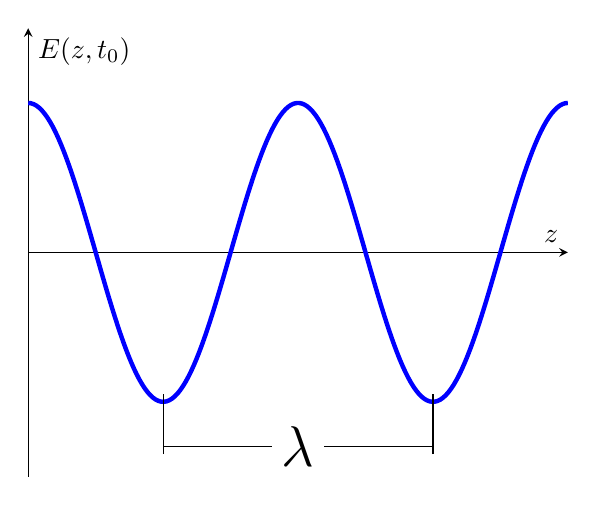
\begin{tikzpicture}
            \begin{axis}[
            axis x line=middle,
            axis y line=middle,
            ymax=1.5,
            ymin=-1.5,
            xmin=0,xmax=pi*4,
            xlabel= $z$,
            ylabel={$E(z,t_0)$},
            yticklabels={,,},
            xticklabels={,,},
            xtick=\empty,
            ytick=\empty,
            ]
            \addplot[domain=0:4*pi,samples=200,blue,ultra thick]{cos(deg(x))};
            \draw (pi,-1.35) -- (pi,-0.95);
            \draw (pi*3,-1.35) -- (pi*3,-0.95);
            \draw (pi,-1.3) -- (pi*3,-1.3) 
            node[pos=.5, fill=white,font=\huge] {$\lambda$};
            \end{axis}
        \end{tikzpicture}        
    \end{center}
    \caption{Plot of E in space}\label{fig:plot_E_space}
\end{figure}

\begin{figure}[H]
    \begin{center}
        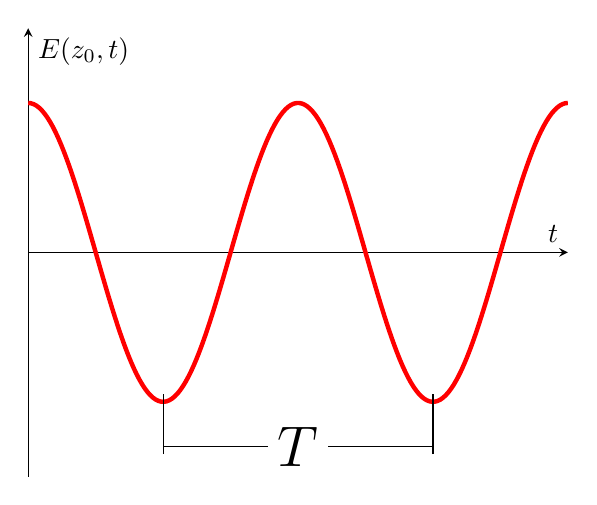
\begin{tikzpicture}
            \begin{axis}[
            axis x line=middle,
            axis y line=middle,
            ymax=1.5,
            ymin=-1.5,
            xmin=0,xmax=pi*4,
            xlabel= $t$,
            ylabel={$E(z_0,t)$},
            yticklabels={,,},
            xticklabels={,,},
            xtick=\empty,
            ytick=\empty,
            ]
            \addplot[domain=0:4*pi,samples=200,red,ultra thick]{cos(deg(x))};
            \draw (pi,-1.35) -- (pi,-0.95);
            \draw (pi*3,-1.35) -- (pi*3,-0.95);
            \draw (pi,-1.3) -- (pi*3,-1.3) 
            node[pos=.5, fill=white,font=\huge] {$T$};
            \end{axis}
        \end{tikzpicture}        
    \end{center}
    \caption{Plot of E in time} \label{fig:plot_E_time}
\end{figure}
We can plot the solution in \cref{eq:maxwell_solution_simple} by considering one of the two variable constant.
\begin{itemize}
    \item \textbf{\cref{fig:plot_E_space}}: if we assume constant time (like if you would take a photograph to the wave) we are evaluating the propagation in space, and so we can obtain the wavelength $\lambda$
    \item \textbf{\cref{fig:plot_E_time}}: if we assume constant space (like if you look the wave from a fixed position) we are evaluating the propagation in space, and so we can obtain the period $T$ 
\end{itemize} 
\subsubsection*{Speed of the wave}
As we said if we plot $E$ in constant time (\cref{fig:plot_E_space}) it is like to take a picture of the wave. If we evaluate the same plot, but in another time point, we can notice that the points of the wave has changed position \cref{fig:plot_E_variation}.\\
From the variation of the space in time we can evaluate the speed of the $E$ wave.
\begin{figure}[H]
    \begin{center}
        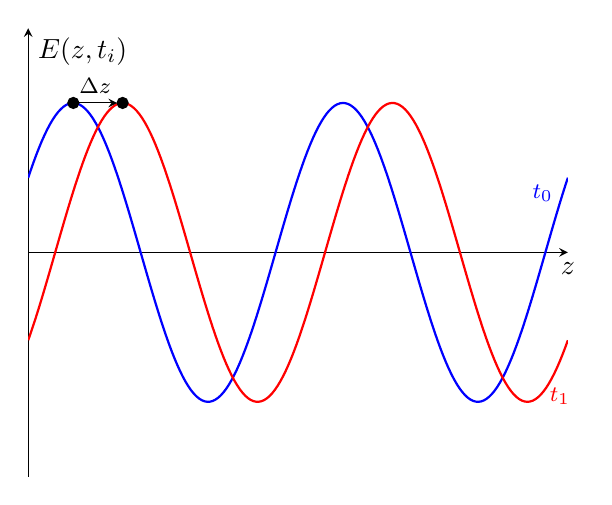
\begin{tikzpicture}
            \begin{axis}[
            axis x line=middle,
            axis y line=middle,
            ymax=1.5,
            ymin=-1.5,
            xmin=0,xmax=pi*4,
            x label style={anchor=north},
            xlabel= $z$,
            ylabel={$E(z,t_i)$},
            yticklabels={,,},
            xticklabels={,,},
            xtick=\empty,
            ytick=\empty,
            ]
            \addplot[domain=0:4*pi,samples=200,blue,thick]{cos(deg(x-pi/3))}
            node[left,pos=.99,font=\footnotesize]{$t_0$};
            \addplot[domain=0:4*pi,samples=200,red,thick]{cos(deg(x-pi*2.1/3))}
            node[right,pos=.95,font=\footnotesize]{$t_1$};
            \addplot [only marks] table {
                2.198 1
                1.05 1
                };
            \draw [stealth-](2.07,1) -- (1.05,1)
            node[midway, above,font=\footnotesize] {$\Delta z$};
            \end{axis}
        \end{tikzpicture}        
    \end{center}
    \caption{Plot of E in two different time}\label{fig:plot_E_variation}
\end{figure}
If we look at \cref{fig:plot_E_variation}, we can assumed that a point of the wave as moved from $z_1$ to $z_2$ from the instant $t_1$ to $t_2$. The function in the two points $(z_1,t_1)$ and $(z_2,t_2)$ has the same relative position (consider to "sit in the wave", you would feel like not moving, but the world around you is moving with a certain speed). So we can write:
\begin{align}
    \begin{split}
        &\omega\left(t_1-\frac{z_1}{c}\right)=\omega\left(t_2-\frac{z_2}{c}\right)\\[5pt]
        &t_2-t_1=\frac{z_2-z_1}{c}\\[5pt]
        &\Delta t= \frac{\Delta z}{c}\\[5pt]
        &c=\frac{\Delta z}{\Delta t}=\frac{\lambda}{T}
    \end{split}
\end{align}
We obtained the propagation speed of the wave:
\begin{equation}
    c=\frac{\partial z}{\partial t}=\frac{1}{\sqrt{\mu \varepsilon}}
\end{equation}
Note that the propagation speed is dependent of $\mu$ and $\varepsilon$, so we can calculate the speed in the vacuum:
\begin{equation}
    c_0=\frac{1}{\sqrt{\mu_0 \varepsilon_0}}=\frac{1}{\sqrt{\frac{1}{36\pi}\cdot 10^{-9}\cdot 4\,\pi\cdot 10^{-7}}}\approx 3\cdot 10^{8}[m/s]
\end{equation}
What we have found is a forward speed because $\Delta z$ is positive and $c$ positive, if we would have used the second equation from \cref{eq:maxwell_solution_simple} the space path $\Delta z$ need to be negative, or we would not be able to have a solution if we try to calculate the propagation speed:
\begin{equation}
    \omega\left(t_1+\frac{z_1}{c}\right)=\omega\left(t_2+\frac{z_2}{c}\right)
\end{equation}
\subsubsection*{Going back to the EMF}
Some more consideration of the EMF
\begin{equation}
    E(z,t)=E_0\,\cos(\omega t-\frac{\omega\,z}{c})
\end{equation}
Now we give some notation for:
\begin{itemize}
    \item $\bm{E_0}$ is the amplitude of the field.
    \item $\bm{\omega=2\,\pi\,\nu } $ is the angular frequency of the EMF
    \item $\bm{\nu =\frac{1}{T}}$ is the frequency of the EMF
\end{itemize}
We can also introduce the phase constant $\bm{\beta=\frac{\omega}{c}}$, and now the wave equation becomes:
\begin{equation}\label{eq:E_with_phase_constant}
    E(z,t)=E_0\cos(\omega\, t-\beta\,z)
\end{equation}
Those two parameters $\omega$ and $\beta$ are useful to obtain the propagation speed.\\
As we have done before, we "take a photo" of the wave (now $\omega t=constant$)and evaluated the propagation speed by considering $(\omega \,t-\beta \,z)$ to be constant, then:
\begin{equation}\label{eq:speed_of_EMF}
    \frac{\partial z}{\partial t}= \frac{\partial }{\partial t}\left(\frac{\omega t}{\beta}\right) = \frac{\omega}{\beta}
\end{equation}
\subsubsection*{Generalization of the EMF}
We can generalize a bit the EMF equation by adding an attenuation constant $\alpha$ and a reference phase $\varphi$
\begin{equation}\label{eq:wave_equation_generalized}
    E(z,t)=E_0\,e^{-\alpha\,z}\cos(\omega\,t-\beta\,z+\varphi)
\end{equation}
$\alpha$ is used to show how the wave is attenuated during his path on the medium.
\subsubsection*{EMF over a general direction}
Usually we consider $\khat$ as the direction of the EMF, but sometimes we need to generalize this direction over all the axes.\\
Consider the forward equation of the EMF over the 3 direction:
\begin{align}\label{eq:electric_field_3_axes}
    \begin{split}
        E(x,t)&=E_0\,\cos(\omega\,t-\beta_x\,x)\\[5pt]
        E(y,t)&=E_0\,\cos(\omega\,t-\beta_y\,y)\\[5pt]
        E(z,t)&=E_0\,\cos(\omega\,t-\beta_z\,z)
    \end{split}
\end{align}
What we do now is to find a way to merge those equation and describe the EMF that goes in a general direction $\overline{r}=x\,\ihat+y\,\jhat+z\,\khat$.\\
In order to do this we introduce the vector $\overline{k}=k_x\,\ihat+k_y\,\jhat+k_z\,\khat$ that generalize the $\beta$ factor, so we can write the wave equation with a general direction:
\begin{equation}
    E(\overline{r},t)=\overline{E}_0\,\cos(\omega\,t-\overline{k}\cdot\overline{r})
\end{equation}
Keep in mind that the direction is not $\overline{r}$ but $\overline{k}$, because $\overline{r}$ represent the variables, and $\overline{k}$ the three weights that defines the direction of the wave.
This is also called the plane wave equation, why?\\
Because we consider $\varphi = 0$ and $\omega\,t=0$ (we take a photo of the wave in $t=0$), so the wave fronts (where E is constant) can be obtained with:
\begin{equation}
    \cancel{\omega\,t}-\overline{k}\cdot\overline{r}+\cancel{\varphi}=-\overline{k}\cdot\overline{r}=k_x\,\ihat+k_y\,\jhat+k_z\,\khat=constant
\end{equation}
Then the last part of the equation is the equation of a plane.\\
Another thing that we can say, is that if $k$ is a scalar value, and $k\,\overline{r}$ is constant, the front of the wave have the shape of a sphere.